This chapter provides important artifacts related to design of our project.

\section{Software Design}

This section presents the UML class diagram and gives a brief description of each class in our system. Attributes and methods of each class and relationship among classes are clearly presented.

\begin{figure}
\caption{UML Class Diagram: The Third Space}
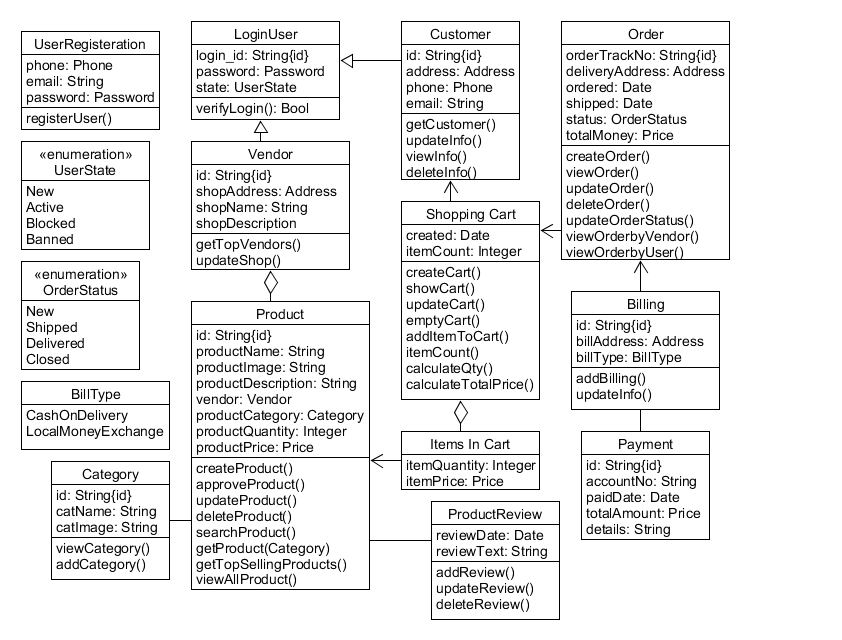
\includegraphics[width=1.25\textwidth]{TheThirdSpaceUML.png} 
\end{figure}


% Your report will contain ONE of the following 2 sections.
\clearpage
\section{Data Design}

This section presents the structure of our database that caters to persistent data storage in our project. The structure is shown as a normalized data model for relational databases. It clearly shows entities, attributes, relationships with their cardinalities, and primary and foreign keys. We have used DB designer (or any other similar data modeling tool) to build our data model.

\begin{figure}[h]
  \caption{ERD: The Third Space}
  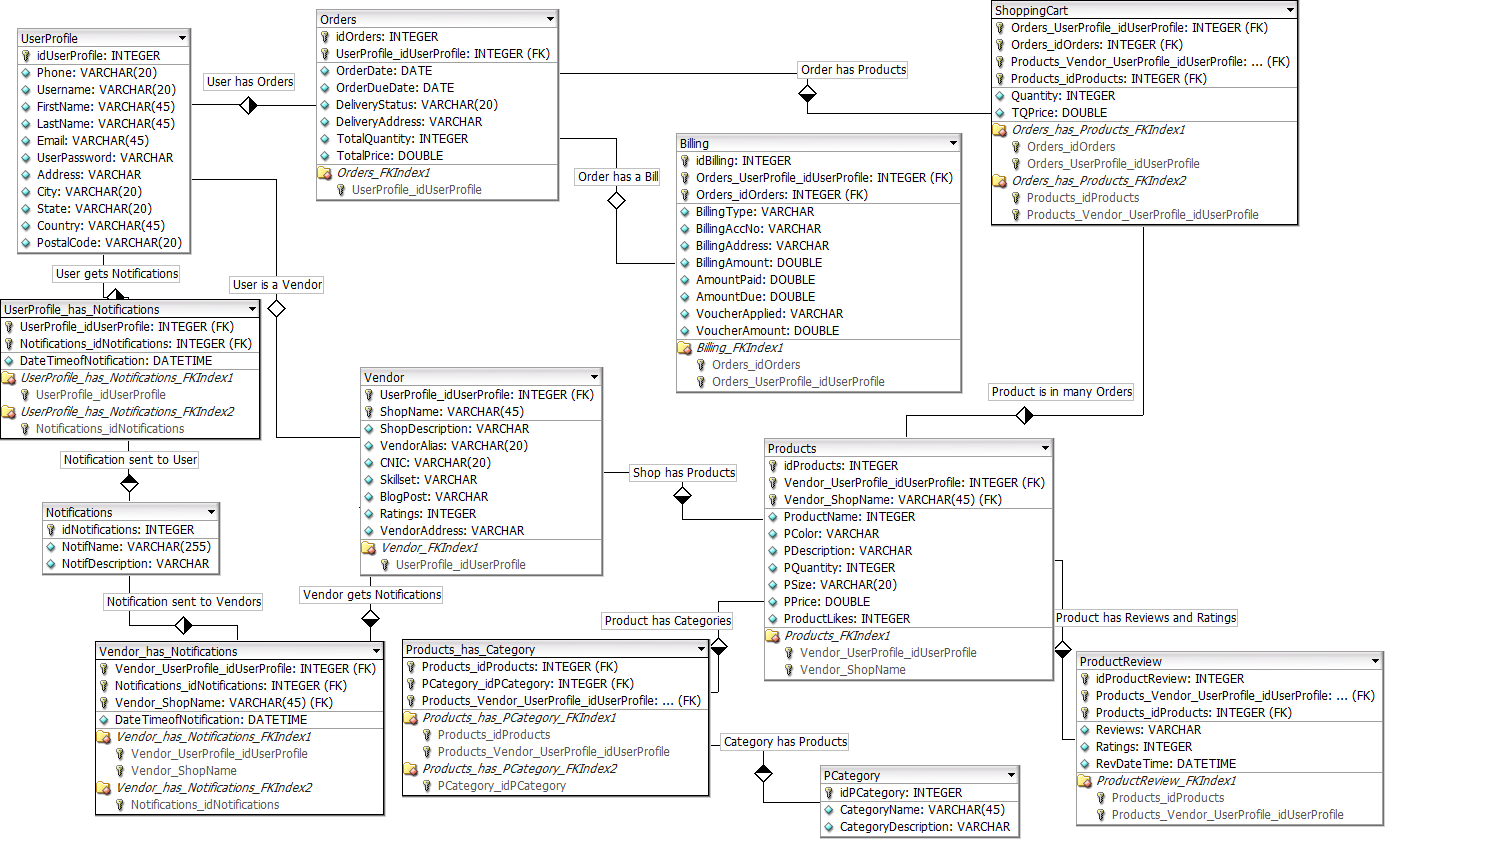
\includegraphics[width=1.25\textwidth]{TheThirdSpaceERD.png}
  \centering
\end{figure}